% THIS IS SIGPROC-SP.TEX - VERSION 3.1
% WORKS WITH V3.2SP OF ACM_PROC_ARTICLE-SP.CLS
% APRIL 2009
%
% It is an example file showing how to use the 'acm_proc_article-sp.cls' V3.2SP
% LaTeX2e document class file for Conference Proceedings submissions.
% ----------------------------------------------------------------------------------------------------------------
% This .tex file (and associated .cls V3.2SP) *DOES NOT* produce:
%       1) The Permission Statement
%       2) The Conference (location) Info information
%       3) The Copyright Line with ACM data
%       4) Page numbering
% ---------------------------------------------------------------------------------------------------------------
% It is an example which *does* use the .bib file (from which the .bbl file
% is produced).
% REMEMBER HOWEVER: After having produced the .bbl file,
% and prior to final submission,
% you need to 'insert'  your .bbl file into your source .tex file so as to provide
% ONE 'self-contained' source file.
%
% Questions regarding SIGS should be sent to
% Adrienne Griscti ---> griscti@acm.org
%
% Questions/suggestions regarding the guidelines, .tex and .cls files, etc. to
% Gerald Murray ---> murray@hq.acm.org
%
% For tracking purposes - this is V3.1SP - APRIL 2009

\documentclass{acm_proc_article-sp}
\usepackage{url}
\usepackage{cite} 
\usepackage{amsmath}
\usepackage{subfigure}
% 中文断行
\XeTeXlinebreaklocale "zh"
\XeTeXlinebreakskip = 0pt plus 1pt minus 0.1pt

% xetex/xelatex 字体设定宏包
\ProvidesPackage{zhfontcfg}
\usepackage{fontspec,xunicode}
\usepackage{CTEX}
%\defaultfontfeatures{Mapping=tex-text} %如果没有它,会有一些 tex 特殊字符无法正常使用,比如连字符。

\usepackage{algorithmicx,algorithm}
\usepackage{algpseudocode}
\usepackage{bm}
\usepackage{graphicx}

\floatname{algorithm}{算法}
\renewcommand{\algorithmicrequire}{\textbf{输入:}}
\renewcommand{\algorithmicensure}{\textbf{输出:}}

\setCJKmainfont[BoldFont={SimHei}]{SimSun}
\setCJKsansfont{KaiTi}
\setCJKmonofont{DengXian}

\begin{document}

\title{{\fontsize{1em}{\baselineskip}\selectfont 人机对弈五子棋AI程序的设计与实现}}

%
% You need the command \numberofauthors to handle the 'placement
% and alignment' of the authors beneath the title.
%
% For aesthetic reasons, we recommend 'three authors at a time'
% i.e. three 'name/affiliation blocks' be placed beneath the title.
%
% NOTE: You are NOT restricted in how many 'rows' of
% "name/affiliations" may appear. We just ask that you restrict
% the number of 'columns' to three.
%
% Because of the available 'opening page real-estate'
% we ask you to refrain from putting more than six authors
% (two rows with three columns) beneath the article title.
% More than six makes the first-page appear very cluttered indeed.
%
% Use the \alignauthor commands to handle the names
% and affiliations for an 'aesthetic maximum' of six authors.
% Add names, affiliations, addresses for
% the seventh etc. author(s) as the argument for the
% \additionalauthors command.
% These 'additional authors' will be output/set for you
% without further effort on your part as the last section in
% the body of your article BEFORE References or any Appendices.

\numberofauthors{2} %  in this sample file, there are a *total*
% of EIGHT authors. SIX appear on the 'first-page' (for formatting
% reasons) and the remaining two appear in the \additionalauthors section.
%
\author{
% You can go ahead and credit any number of authors here,
% e.g. one 'row of three' or two rows (consisting of one row of three
% and a second row of one, two or three).
%
% The command \alignauthor (no curly braces needed) should
% precede each author name, affiliation/snail-mail address and
% e-mail address. Additionally, tag each line of
% affiliation/address with \affaddr, and tag the
% e-mail address with \email.
%
% 1st. author
\alignauthor
赵乙宁\\
       \affaddr{2017010435}\\
       \email{zhaoyn17@mails.tsinghua.edu.cn}
% 2nd. author
\alignauthor
余齐齐\\
       \affaddr{2018013361}\\
       \email{yqq18@mails.tsinghua.edu.cn}
}

\maketitle

\begin{abstract}
基于Minimax搜索和$\alpha$-$\beta$优化剪枝的方法,我们编写了一个可进行人机对弈的AI程序。程序从当前状态开始,
依次考虑双方每一种可能动作及其引起的结果状态,对由此产生的状态树进行深度优先的搜索,并使用启发式方法对状态进行估值,和适当
的剪除不必要搜索的分支,从而减小计算量和提高效率。\\
除此之外,我们还使用了散列记录搜索过程中找到的结点的搜索结果,以避免重复搜索相同局面;使用迭代深度搜索方法以充分利用有限的
时间完成尽可能多的搜索,并让浅层的搜索结果为高层的搜索提供子节点搜索顺序的参考。
根据五子棋的特点,我们还引入了一种特别的搜索顺序和剪枝方法:优先搜索距离前几步下棋位置近的结点、剪除距离任何现有棋子都很远
的结点,以进一步降低搜索树的平均分支数,加快搜索效率、加深在有限时间内可以搜索到的层数。
最后,我们在现有框架的基础上加入了悔棋和复盘的功能,丰富了游戏的提示文字、完善了输入检查,以增强人类玩家使用本程序的体验。\\
在实验环境下,我们的程序可以在$5s$内搜索平均$2.5\times10^6$个结点,对状态树完整地完成$4-6$层的搜索。程序在与人类的实际对战中
也取得了良好的效果,有时可以提前5-8回合就找到制胜的策略。\\
       \\
\end{abstract}

\section{\textbf{概述}}
我们使用了常用的对抗搜索方法——Minimax搜索,即交替模拟双方可以采取的最优动作;并使用$\alpha-\beta$优化剪枝的方法
降低搜索的分支数,提高搜索的效率。\\
由于五子棋在任何一个空位置下棋都是合法的行动,五子棋问题的搜索树的平均分支数量极高,
可以达到近200,而游戏结束往往需要30-60轮行动,因而不可能一次性搜索到最终游戏结束的结点状态,
故使用启发函数评估局面的限定深度搜索是必须的。根据五子棋的特点,我们使用了一套启发式评估方法,它评估双方在场上拥有的活二、
活三、冲三、活四、冲四等棋型的数量,并以此为依据对局面做出预估。\\
此外我们还是用迭代深度搜索和散列表优化的方法,以最大限度的利用所给的时间进行尽可能深入的搜
索,避免重复搜索已经搜索过的状态,以及优化了子结点的搜索顺序、提高了$\alpha-\beta$优化剪枝的效果。\\
根据五子棋的特点,我们还引入了基于距离的优化方法:先搜索距离前几个回合下棋位置近的节点,和剪除距离棋盘上任何棋子都较远的空位置位置的搜索,
以进一步的提高剪枝的效果、降低搜索树平均
分支数量,从而提高搜索效率、加深搜索层数的目的。\\
我们的程序不仅实现了人机对弈所需要的基本功能,还额外实现了悔
棋、复盘等附加功能,并有丰富的文字提示和完善的输入法性检查,以给人类玩家使用本程序带来更好的体验。\\

\section{\textbf{搜索算法的设计与实现}}

\subsection{\textbf{程序基本框架}}
总体上程序可以分为两个部分:通用五子棋运行逻辑部分和AI智能体部分,前者负责从控制台读取人类玩家的输入、调用AI智能体部分提供的接
口获取AI的输入,合法性验证、判断游戏是否结束,和控制棋盘的打印、悔棋、存盘、复盘等;后者则为通用五子棋运行逻辑部分提供一个接口,
接受某一时刻的棋盘等游戏状态信息,并返回一个AI此时希望下棋的位置。详细的文件模块介绍如表1所示。\\
\begin{table*}
        \small
       \centering
       \caption{文件模块一览表}
       \begin{tabular}{|c|c|l|} \hline
       所属部分 & 文件名(不含扩展名) & 说明\\ \hline
       运行逻辑 & define & 定义各类基础的游戏数据结构如棋盘、点、行棋记录、启发式估值等\\ \hline
       运行逻辑 & start & 游戏主循环,控制复盘、存盘、读取人类和AI的动作输入、打印棋盘等\\ \hline
       运行逻辑 & makemove & 解析控制台输入,获取AI输入,验证合法性,进行下棋,撤销下棋\\ \hline
       运行逻辑 & gameover & 判断游戏是否结束和胜负\\ \hline
       运行逻辑 & printchessboard & 把棋盘打印在控制台上\\ \hline
       AI & evaluate & 对一个完整游戏状态进行局面估值\\ \hline
       AI & createmoves & 产生所有的可行动作和循环遍历时的先后顺序构成的有序列表\\ \hline
       AI & searchmove & 对局面进行递归的、迭代深度的Minimax搜索和$\alpha-\beta$优化剪枝\\ \hline
       AI & hashsearch & 定义散列表,提供接口计算局面的键值、修改和查询散列表中的数据\\ \hline
       AI & cutoffTest & 判定是否停止搜索子节点、调用启发式函数对局面进行估值\\ \hline
       AI & stopSearchSiblingsTest & 判定是否因$\alpha-\beta$或超时等,对未搜索的子结点进行剪枝\\ \hline
       \end{tabular}
\end{table*}


\subsection{\textbf{Minimax搜索和$\alpha-\beta$优化剪枝}}
基本的Minimax搜索方法是用递归函数来实现的,在我们的程序中对应于searchmove.cpp的SearchStep函数。\\
一个很重要的事实是,$\alpha-\beta$算法的效果受到搜索子结点的先后顺序的影响十分严重,下面将对此作出分析。\\
算法在搜索当前玩家为AI的结点($status.player\ ==\ $black)时,会从所有子节点返回的搜索结果中选择分数最大的一
个作为本结点返回的搜索结果;反之在搜索当前玩家为人类的结点时则选择分数最小的子节点。\\
设$A$为一个当前玩家为AI的结点,$B_1, B_2, \dots , B_n$为它的子结点(显然它们的当前玩家均是人类)。那么如果记已经搜索完
成 的$B_1, B_2, \dots , B_k-1$所返回的分数的最大值为$\alpha$,随后在进入$B_k$结点、循环遍历$B_k$的子结点的过程中,一旦
发现任何子结点的值$\leq \alpha$,那么因为$b_k$会返回它的所有子结点的返回值的最小值,$b_k$最终返回的值必然也$\leq \alpha$,
从而就不可能成为$A$的子结点搜索结果的最大值,也就不可能成为对$A$结点的搜索的返回值。既然如此,我们就可以直接结束对$B_k$
结点的搜索,这就是$\alpha-\beta$优化剪枝的基本原理。\\
分析可以知道,在$B_k$结点之前被搜索完成的结点的分数越高,那么$B_k$结点就越容易被剪枝,因此提高Minimax\ $\alpha-\beta$算
法的性能的关键就在于在对每一个结点的搜索过程中,都让能产生最优结果的子结点被尽可能早的搜索。为此,我们引入了多种方法来优
化结点的搜索顺序,详见下文所述。

\subsection{\textbf{散列表优化和迭代深度搜索}}
为了进一步优化程序,我们使用了散列表优化\cite{xqbase1}和迭代深度搜索\cite{xqbase3}两种方法。\\
散列表优化是在搜索的过程中,对完成搜索的每一个结点,将该结点的游戏状态、搜索层数、搜索结果分数和对应的最优行动等信息存储
在散列表中。对于一个散列表而言,在其上存储一个数据和查找一个已经存在于其上的数据的时间复杂度均为$O(1)$,因而对于
随机增删和查找的场景有着很好的适用性。但是利用散列表存储的前提是需要对棋局的状态产生一个整形的数值(称为键值)来描述它,
这里我们选用的是Zobrist键值。\cite{xqbase2}
Zobrist键值通过为棋盘上的每个位置、每个棋子分配64位随机整数,通过异或运算产生键值,能够实现当在棋盘上放置或撤下单颗棋子时
可以在$O(1)$的时间内完成键值的计算,因而与需要遍历整个棋盘才能计算完成的键值计算算法相比具有很大的优势。\\
在散列表方面,出于效率考虑,我们使用了C++标准库std::unordered\_set,并在游戏开局前预先调整其内的散列表大小为3M,从而可以
获得最优的效率。\\
此外在现实中,智能体做出决策的时间是有限的。为了充分的利用
给定的时间,我们引入了迭代深度搜索:如果限定深度为$k-1$的搜索完成时给定的时间没有用尽,
则立即开启一个限定深度为$k$的搜索;在搜索的检查耗时,如果发现时间已经用尽则搜索函数立刻提前返回。\\
但更重要的其实是,迭代深度搜索与散列表的结合有利于在后续的搜索过程中更好的优化子结点的搜索顺序。通常来讲,如果一个动作在浅层的搜索中被找
到作为最优的行动,那么当搜索层次加深时,从概率的角度上,它仍然是深层搜索得到的最优行动的概率是很大的。因此,我们只需要在散
列表的表项中同时保存搜索结果的分数和行动两项数据,即可以在深层搜索中查到到刚刚浅层搜索所找到的最优行动并优先搜索。\\
综上所述,散列表中的数据内容定义如下:
\begin{quote}
    \small
       struct HashTableItem \{\\
              \hspace*{0.6cm} unsigned long long zobrist; // zobrist键值 \\
              \hspace*{0.6cm} int depth; // 该搜索记录产生时对应的深度 \\
              \hspace*{0.6cm} int score; // 搜索结果的分数 \\
              \hspace*{0.6cm} int scoreType; // 分数的类型,有准确结果、alpha结果、beta结果三种可能 \\
              \hspace*{0.6cm} Point bestMove; // 搜索结果对应的行动的下棋位置 \\
       \};
\end{quote}

\subsection{\textbf{基于距离的合法行动有序列表的产生、排序(CreateMoves模块)与剪枝}}
五子棋的一般经验表明,在大多数情况下效用高的下棋位置要么是偏向进攻的,即延长自己已经有的连珠使其接近五连珠;
要么是防守的,即破坏、截断对手的连珠,避免其在未来成为五连珠。无论哪种情况,我们往往都在自己现有的棋子周边或对方现有
的棋子周边下棋,而一般不会在距离任何现有棋子都很远的空位置下棋。进一步的如果考虑到局势的进展,往往在一个“交战中心”,即双方
最近几回合下棋位置的附近下棋得到的效用是相对高的。\\
因此,在产生合法行动的有序列表和安排它们的初始搜索顺序时,我们计算每个空位置到最近两回合的下棋位置的距离最小值,并进行升序
排列产生搜索顺序,如算法1所示。\\
\begin{algorithm}
    \algsetup{\tiny}
    \scriptsize
    \caption{产生合法行动的有序列表}
    \begin{algorithmic}[1] %每行显示行号
        \Require 当前完整状态$status$(包括棋盘$status.board$、当前行动玩家$status.player$等、历史记录$status.history$等)
        \Ensure 所有合法行动组成的有序列表$result$
        \Function {MakeMoves}{$status$}
        \State $historyPoints = \{status.history[-1], status.history[-2]\}$
        \State $emptyPlaces = $棋盘上的所有空位置
        \ForAll {$place$ in $emptyPlaces$}
        \State 计算到$historyPoints$的距离的最小值$place.priority =\ $\Call{minDistanceTo}{$place, historyPoints$}
        \EndFor
        \State 按priority排序所有空位置$result =\ $\Call{SortByPriority}{$emptyPlaces$}
        \State \Return {$result$}
        \EndFunction
    \end{algorithmic}
\end{algorithm}
上述的排序方法没有从根本上减小最坏情况下一个结点的分支数。然而分析可以知道,在最顶层结点处
的$\alpha=-\infty, \beta=-\infty$,因此最顶层结点是必定会完成对所有子结点的遍历的,因此从根本上减小最坏情况结点的分支数
对提高搜索效率有着重要的意义。事实上
在大多数情况下,很少有一步效用很高的棋是远离棋盘上任何现有棋子的,因为这样的棋既不能起到进攻也不能起到防守的作用。因此可以
在搜索时对某个空位置,判断其周边与其距离$\leq2$的范围内是否已有任何棋子,如果没有则跳过对这个
空位置的搜索。\\

\subsection{\textbf{搜索算法的最终实现(SearchMove模块)}}
AI智能体部分对外提供一个接口SearchMove(),它返回一个Point结构体,其中包括x、y两个int类型的数据,代表一个点的坐标。\\
SearchMove()函数没有形参,但是会读取define.h中定义的游戏棋盘、当前玩家、游戏历史记录等数据,组合成GameFullStatus类的对象;
随后用一个循环迭代深度地调用SearchStep函数,由此开始对状态树的根节点(即当前局面)的搜索。\\
而对状态树的搜索的核心在于SearchStep函数。SearchStep函数的一次调用表示对一个结点的完整搜索过程,其内部主要的内容包括产生
合法行动的有序列表,用循环遍历这个列表、依次执行每个行动产生子状态,递归调用SearchStep搜索子状态结点,最后返回所有子状态
的结果中最优的一个。其具体的算法如算法2所述。\\
\begin{algorithm}
    \algsetup{\tiny}
    \scriptsize
    \caption{搜索单个状态结点}
    \begin{algorithmic}[1] %每行显示行号
        \Require 当前完整状态$status$(包括棋盘$status.board$、当前行动玩家$status.player$等)、当前剩余深度$depth$
        、上层$\alpha$、上层$\beta$
        \Ensure 搜索结果$result$(包括评估分数$result.score$、对应哪个合法动作$result.move$)
        \Function {SearchStep}{$status, depth, \alpha, \beta$}
        \If {$depth == 0$}
        \State 调用启发函数评估分值$result.score = $\Call{evaluate}{$status$}
        \State \Return{$result.score$}
        \EndIf
        \State 产生所有合法行动的有序列表$legalMoves = $\Call{makemoves}{$status$}
        \If {散列表存在一个项$item$,其对应的键值与当前状态相同}
        \If {$item.depth \geq depth$}
        \State \Return{item.score & item.bestMove}
        \Else
        \State 将$item.bestMove$在$legalMoves$中的位置移动到最开头
        \EndIf
        \EndIf
        \If{$status.player ==\ $black}
        \State $result.score = -\infty$
        \ForAll {$legalmove$ in $legalmoves$}
        \State \textbf{if}\ 到棋盘上任意其他棋子的最短距离\Call{minDistanceToAnyChess}{$legalmove$} $\ge2$ \ \textbf{then}\ \textbf{break}
        \State $status.$\Call{putChess}{$legalmove$}
        \State $curRes = $ \Call{SearchStep}{$status, depth - 1, \alpha, \beta$}
        \State $status.$\Call{unputChess}{$legalmove$}
        \State \textbf{if}\ {已经超时} \ \textbf{then}\ \textbf{break}
        \If {$curRes.score > result.score$}
        \State $result = curRes$
        \State $\alpha = $ \Call{max}{$\alpha, result.score$}
        \EndIf
        \State \textbf{if}\ {$result.score >= \beta$} \ \textbf{then}\ \textbf{break}
        \EndFor
        \EndIf
        \If{$status.player ==\ $white}
        \State $result.score = +\infty$
        \ForAll {$legalmove$ in $legalmoves$}
        \State \textbf{if}\ 到棋盘上任意其他棋子的最短距离\Call{minDistanceToAnyChess}{$legalmove$} $\ge2$ \ \textbf{then}\ \textbf{break}
        \State $status.$\Call{putChess}{$legalmove$}
        \State $curRes = $ \Call{SearchStep}{$status, depth - 1, \alpha, \beta$}
        \State $status.$\Call{unputChess}{$legalmove$}
        \State \textbf{if}\ {已经超时} \ \textbf{then}\ \textbf{break}
        \If {$curRes.score < result.score$}
        \State $result = curRes$
        \State $\beta = $ \Call{min}{$\beta, result.score$}
        \EndIf
        \State \textbf{if}\ {$result.score >= \beta$} \ \textbf{then}\ \textbf{break}
        \EndFor
        \EndIf
        \State \Return{$result$}
        \EndFunction
    \end{algorithmic}
\end{algorithm}


\subsection{\textbf{启发式函数}}
在现实情况中,应该在合理的时间内做出决策。为实现此目的,应尽早截断搜索,将启发式评估函数用于搜索中的状态,有效的将非终止结点转变为终止结点。\\
启发式搜索如下:\\
\begin{tiny}
HMinmax(s,d)=\\
\begin{equation}
\begin{split}
\begin{aligned}
\left\{
\begin{array}{lr} 
EVAL(s),& if CutoffTest(s,d), \\
max_{a\in Actions(s)}HMinmax(Result(s,a),d+1) , & player(s)=MAX,\\
min_{a\in Actions(s)}HMinmax(Result(s,a),d+1), & player(s)=MIN.
\end{array}
\right.
\end{aligned}
\end{split}
\end{equation}
\end{tiny}
\\
在五子棋人机对弈中,启发式函数可以通过对关键棋型的统计来得到局面形势估计值,某一方的关键棋型越多,在对弈中更有主动权,优势也就更大。\\
\subsubsection{\textbf{关键棋型介绍}}
五子棋中的基本棋型有连五、活四、冲四、活三、眠三、活二(眠二对局面影响很小,此处不计入)。\\
1.连五棋型,此时已经可以判断胜负,示例如下图。\\
2.活四棋型,有两个连五点,示例如下图。\\
3.冲四棋型,只有一个连五点,示例如下图。\\
4.活三棋型,可以连成活四的三,示例如下图。\\
5.眠三棋型,可以连成冲四的三,示例如下图。\\
6.活二棋型,可以连成活三的二,示例如下图。\\

\begin{figure}[htbp]
	\centering
	\subfigure[连五棋型]{
		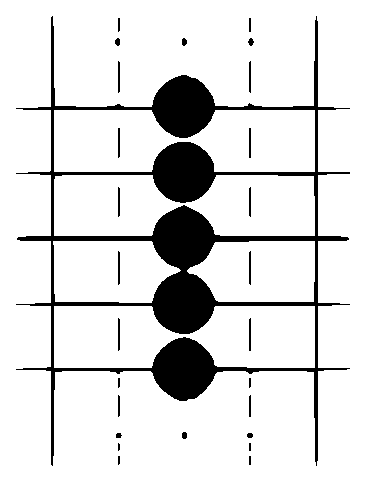
\includegraphics[height=0.6in, width=0.7in]{chessMode5.eps}
		%\caption{fig1}
	}
	\quad
	\subfigure[活四棋型]{
		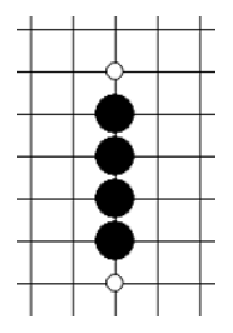
\includegraphics[height=0.5in, width=0.7in]{chessModeL4.eps}
	}
	\quad
	\subfigure[眠四棋型]{
		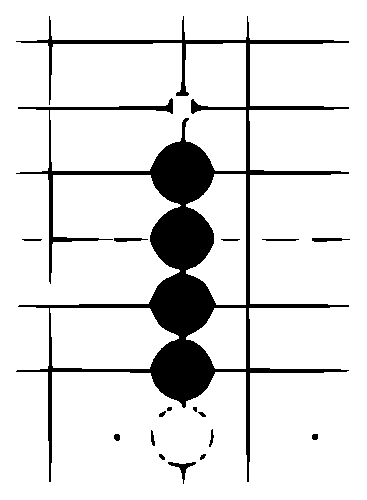
\includegraphics[height=0.5in, width=0.7in]{chessModeS4.eps}
	}
	\quad
	\subfigure[活三棋型]{
		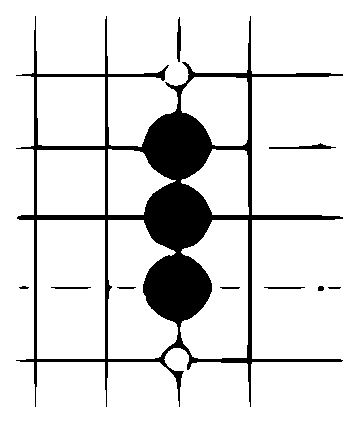
\includegraphics[height=0.5in, width=0.7in]{chessModeL3.eps}
	} 
	\subfigure[眠三棋型]{
		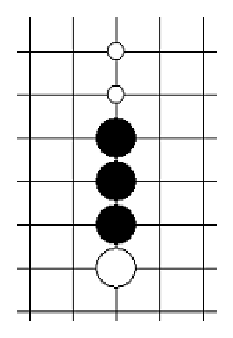
\includegraphics[height=0.5in, width=0.7in]{chessModeS3.eps}
	} 
	\subfigure[活二棋型]{
		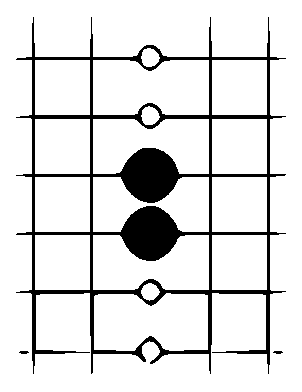
\includegraphics[height=0.5in, width=0.7in]{chessMode2.eps}
	}
\end{figure}

\subsubsection{\textbf{棋型统计策略}}
对棋子进行遍历,棋子有可能在四个方向()从左到右,从上到小,从左上到右下,从右上到左下)上形成基本棋型,对四个方向进行搜索,每个方向取以该棋子为中心的9个位置,得到位置数组,对这个数组进行棋型搜索,即可得到该棋子形成的所有棋型数目。\\
需要注意的是,为了防止棋型的重复计入,我们需要记录已经被标记过的棋盘位置,下一次遍历到此位置时便不再查找此棋子附近形成的棋型。\\
\begin{tiny}
\begin{algorithm}
       \algsetup{\tiny}
       \scriptsize
	\caption{棋型统计策略}
	\begin{algorithmic}[1] %每行显示行号
		\Require  当前棋盘 $board$、当前棋子坐标$(i,j)$、方向数组$dir_s$
		\Ensure  该棋子形成的棋型数目数组$count[]$ 当前棋盘 $board$
		\Function {EvaluatePoints}{}
		\If {该棋子未被记录过}
	 	\ForAll {direction in 方向数组 $dir_s$}
	 	\State 调用得到以该棋子为中心该方向上的9个位置的数组  line= getline(board,i,j);
	 	\State 对line数组进行搜索,得到该棋子形成的棋型数目数组count;
	 	\State
	 	记录与该棋子共同形成棋型的己方棋子坐标
		\EndFor
		\State	\Return 该棋子形成的棋型数目数组count;
		\EndIf
		\EndFunction
	\end{algorithmic}
\end{algorithm}
\end{tiny}

\subsubsection{\textbf{局面估值策略}}
当我们对棋局的所有棋子进行了棋型统计之后,我们便容易得到黑棋和白棋的基本棋型的数目总值。局面的估值应该是己方棋型权值与对方棋型权值的差。\\
根据棋型的数目进行局面估值有两种策略,一种是对能够在几步之内分出胜负的棋型,也就是必杀,对这种棋型,我们直接返回一个较大的对局面的估值;一种是在当前情况下暂时没有办法分出胜负的棋型,对这种的棋型,我们通过统计基本棋型的数量,与设置的棋型权值相乘,返回权值和。对这两种棋型的区分可以优化后续搜索的层数。\\
值得注意的是,下棋的顺序会影响到局面的估值,若当前是黑棋的回合,黑棋还未下,而白棋已经下过,那么相同的棋型白棋和黑棋的估值应该就有所不同。例如,白棋有活三,黑棋有活三,此时黑棋不构成必杀,但白棋显然构成必杀,因为白棋下一步就可以将活三变为活四。\\
基于以上考虑,在启发式函数中,我们将棋型估值设置如“表格-棋型估值”所示。\\
注意:必杀的招数按照权值从大到小进行判断,再返回权值,这样可以直接解决多个必杀棋型的优先级的问题。对于黑白两方都有连五的棋型,逐步撤销已下棋子,递归到只有一方连五判断。\\

\begin{table}
    \small
	\centering
	\caption{棋型估值}
	\begin{tabular}{|c|l|} \hline
	黑棋连五 & 1000000 \\ \hline
	 白棋连五 &- 1000000 \\ \hline
	 白活四 &- 9050 \\ \hline
	 白冲四 &- 9040 \\ \hline
	 黑活四(黑棋两冲四相当于一活四) &9030 \\ \hline
	 黑冲四活三& 9020 \\ \hline
	 黑无冲四白有活三 &-9010\\ \hline
	 
	 黑有两活三白无活三或眠三& 9000 \\ \hline
	基本棋型()不构成必杀 &  权值\\ \hline
	 黑冲四 &  400\\ \hline
	 白眠三 &  400\\ \hline
	 黑活三 &  100\\ \hline
     黑眠三 &  80\\ \hline
     白活二    &  80\\ \hline
     黑活二     &  40\\ \hline
	\end{tabular}
\end{table}

\subsection{\textbf{游戏结束的判断(GameOver模块)}}
在每一次下棋后,立刻在八个方向、距离为4的范围内查找与刚刚被下的棋子连续的同一方棋子的个数,从而计算出是否有五连珠。由于
每一回合下棋后都会进行这一判断,因此这一方法足以准确判断出游戏是否结束的结果。另外,若棋盘下满无人胜利,则判断为和棋。
\subsection{\textbf{悔棋和复盘的实现}}
维护一个下棋历史数组。悔棋时,撤销最后下的两手棋,数组弹出元素,更新棋盘。\\
将复盘的下棋历史存储在同目录的ChessSave.txt下,每次棋局结束时,提示是否要存盘,若存盘则将下棋历史存储在ChessSave.txt中,
每次棋局开始时,提示是否要复盘,若需要复盘则播放ChessSave.txt中的历史记录。\\

\section{\textbf{实验}}
衡量基于对抗搜索的算法的优劣的重要标准,就是在规定时间内算法完成搜索的层数,因为更多的搜索层数往往意味着对更远的未来形势的预测,
往往在实际的人机对弈中有着更好的效果。\\
在实验环境:Intel Core i7-7500U 2.90GHz,Windows 10 64bit,GCC 8.1.0 64位Release编译的实验条件下,我们调整程序中各个模块
的开关,测试其在5s内完成搜索的完整层数和搜索的结点个数,结果如表3所示。\\
由于需要限定时间,迭代深度搜索在各个实验中均
开启,但在不开启散列表的情况下由于无法记忆浅层搜索的结果,迭代深度搜索不会起到优化顺序的作用。其余的模块在表3第一列对应的序号为:
0:Minimax,1:$\alpha-\beta$剪枝,2:散列表,3:基于距离的搜索顺序优化,4:基于距离的空位置剪枝。\\
表3第二列的层数表示5s内所能够完整搜索完成的层数,不包括由于超时而中途退出、没能完整搜索的层数;第三列的结点数表示5s内所能够搜索
的状态树的结点个数;第四列的胜率表示笔者本人与该AI进行对战,始终是笔者先手的情况下,与其多次对战的大致胜率。\\
\begin{table}
    \small
    \centering
    \caption{不同模块配置下的程序搜索效率}
    \begin{tabular}{|l|c|c|c|} \hline
    模块配置 & 层数 & 结点数 & 胜率\\ \hline
    0 & 2 & 4800000 & ~20\% \\ \hline
    0+1 & 3 & 3900000 & ~70\% \\ \hline
    0+1+2 & 3-4 & 2600000 & ~80\% \\ \hline
    0+1+3 & 4 & 3200000 & ~100\% \\ \hline
    0+1+2+3 & 4 & 2100000 & ~100\% \\ \hline
    0+1+2+3+4 & 5-6 & 1500000 & ~100\% \\ \hline
    \end{tabular}
\end{table}
观察表格可以知道,随着开启模块的不断增多、算法的不断变复杂,在5s内能够搜索结点的个数是下降的,这是因为开启的模块越多,对应的
搜索单个结点时的计算量也就越大。但是实际完整搜索的层数却呈现完全相反的态势:开启的模块越多,则进行剪枝优化的效果就越好,从而能够
达到更深的搜索深度。特别是我们自行引入的、基于空位置到最近棋子的距离剪枝的方法,可以非常明显的增加搜索能够达到的层数,起到了很好的剪枝效果。\\
而在与人对战方面,本程序也有着很好的效果。表格第四列是使用该程序与笔者进行对战(笔者先手)时候,AI一方的大致胜率。可以看出
大体上搜索能够达到的深度越深,与人对战的效果越好。\\
此外对最终版本(0+1+2+3+4),我们还邀请了多名亲友与之对战,合计大约30局左右,人类无一胜绩。这表明我们的AI在五子棋方面已经有了
一定的与人对战的能力。

\section{实验收获与体会}
在设计和实现人机对弈五子棋AI的过程中,我们对Minimax搜索、$\alpha-\beta$优化剪枝、启发式函数、迭代深度搜索有了更加全面和深入的了解。\\
在早期粗略的设计实现后,AI其实已经可以实现基本的对弈功能了,但它的下棋总会非常的奇怪:不去堵对方的成三、下的位置常常让人摸不着头脑。于是我们不断的去优化它——加入了优化剪枝、迭代深度搜索让它能够搜索的步数更多,修改启发函数让它能在较小的时间内能够做出较优的判断,也实验了一种优化方法——舍弃掉““荒郊野岭”即距离棋子较远的位置,想法是在交战中心作战是更有效率的方法,实验之后,效率得到了相当大的优化。\\
在设计的过程中,我们认识到了对抗搜索方法的优越性,也体会到了先验知识的重要性,启发式函数、结合游戏实际的优化策略往往能够使决策变得更高效。\\
五子棋与其他棋类游戏如围棋相比,是相对简单的,与生活实际中的很多决策情境相比更是不值一提,人工智能如何能够在更复杂的情境下更高效的完成任务呢?我想我们还要继续学习。\\
最后非常感谢老师和助教的指导!\\

%ACKNOWLEDGMENTS are optional
%
% The following two commands are all you need in the
% initial runs of your .tex file to
% produce the bibliography for the citations in your paper.
\small
\bibliographystyle{abbrv}
\bibliography{sigproc}
% That's all folks!
\end{document}
